\documentclass[12pt]{article}

\usepackage[english]{babel}
\usepackage[utf8x]{inputenc}
\usepackage{pdfpages}
\usepackage{lastpage} % Required to determine the last page for the footer
\usepackage{extramarks} % Required for headers and footers
\usepackage{graphicx} % Required to insert images
\usepackage{listings} % Required for insertion of code
\usepackage{courier} % Required for the courier font

% Margins
\topmargin=-0.45in
\evensidemargin=0in
\oddsidemargin=0in
\textwidth=6.5in
\textheight=9.0in
\headsep=0.25in

\linespread{1.1} % Line spacing

\newcommand{\Title}{Design Documentation} % Assignment title
\newcommand{\Class}{Cos\ 301} % Course/class

\begin{document}

	\vspace{4em}
	
	\begin{center}%
	
	  \LARGE \bf \Title \\[4em]
	  \LARGE {\bf Group 1}\\[1em]
	  \LARGE {\bf Group Members:}\\[2em]
	  \large
	  
	     Mbulungo Musetsho				(10176382) \\[1em]
	     Ndivhuwo Ntambeleni			(10001183) \\[1em]
	     Pule Legodi                                (29302732) \\[1em]
	    	%Enter your details below just as the one above
	    
	\end{center}%
	

	\newpage
	\tableofcontents
	
	\newpage
	\section{Background}
	
		\vspace{0.2in}
	
				 %We must give an introduction of this document
		
		 
	
	\section{Vision}
	
		\vspace{0.2in}
		
			 		 %We must briefly describe the purpose of this document
				
	
	\section{Software Architecture Design}
			%This section needs to demonstrate how the system will be able, within designed software architecture, to address the non-functional requirements.
		\vspace{0.2in}
		
		\subsection{Choices of Technologies}
		%Please refer to the guideline document for some of the items that must be included in this part.
			\vspace{0.2in}
		
		
		\subsection{Chosen Frameworks}
				%Please refer to the guideline document for some of the items that must be included in this part.
					\vspace{0.2in}	
			
		
		\subsection{Chosen Protocols}
				%Please refer to the guideline document for some of the items that must be included in this part.
		
			\vspace{0.2in}
			
		
		\subsection{Chosen Libraries}
				%Please refer to the guideline document for some of the items that must be included in this part.
			\vspace{0.2in}

			
	\section{Application Design}
				%must address functional requirements as specied in re-quirements specification.
			\vspace{0.2in}
					
		\subsection{Lower Levels of Granularity Specification}
				
		\vspace{0.2in}
		
		\subsection{API Specifications}
						%UML interfaces and class diagrams for inputs and outputs, etc
				\vspace{0.2in}
				
		\subsection{System Class Diagrams }%Ndivhuwo Nthambeleni
		%Class Diagram for assessment marking and assessment aggregation
				
				\begin{figure}[ht!]
						\centering
						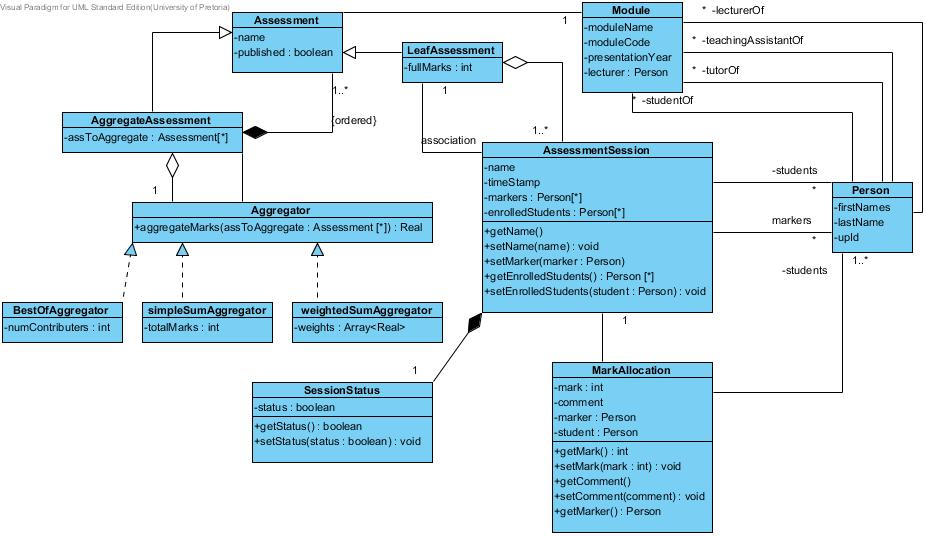
\includegraphics[width=2in, height=2in]{Pictures/MiniPhase2ClassDiag.jpg}
						\caption{Assessment Class Diagram}
				\end{figure}
						%These class diagrams must include attributes, methods and relationships
						
				\vspace{0.2in}
		
		\subsection{System Process Specification}%Mbulungo Muusetsho
						%Sequence and activity diagrams for detailed system process specifications
						\begin{figure}[h]
										\centering
										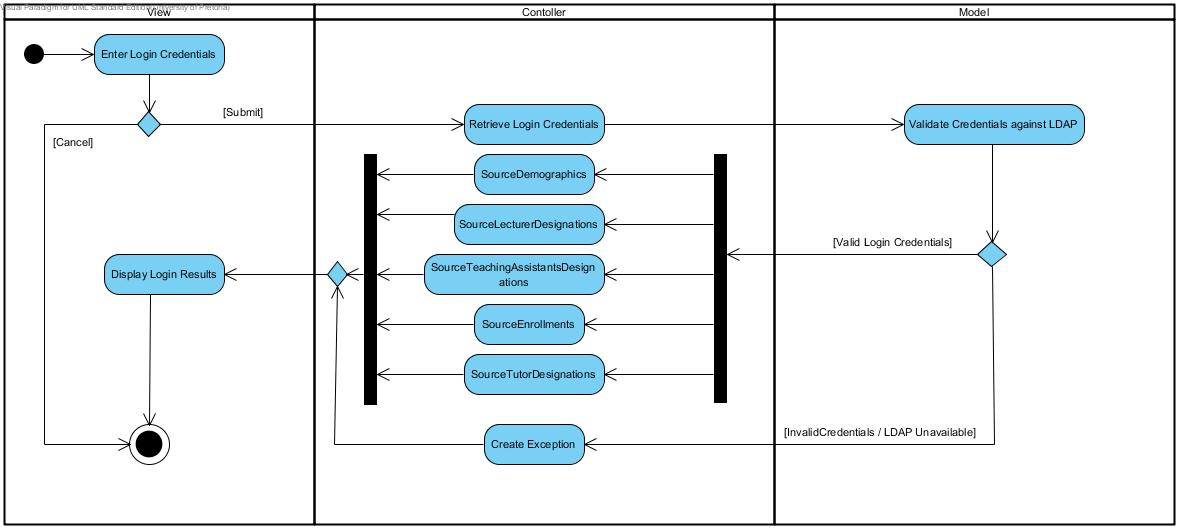
\includegraphics[width=2in, height=2in]{Pictures/LoginActivityDiagram.jpg}
										\caption{User Log In Activity Diagram}
						\end{figure}
						\begin{figure}[h]
										\centering
										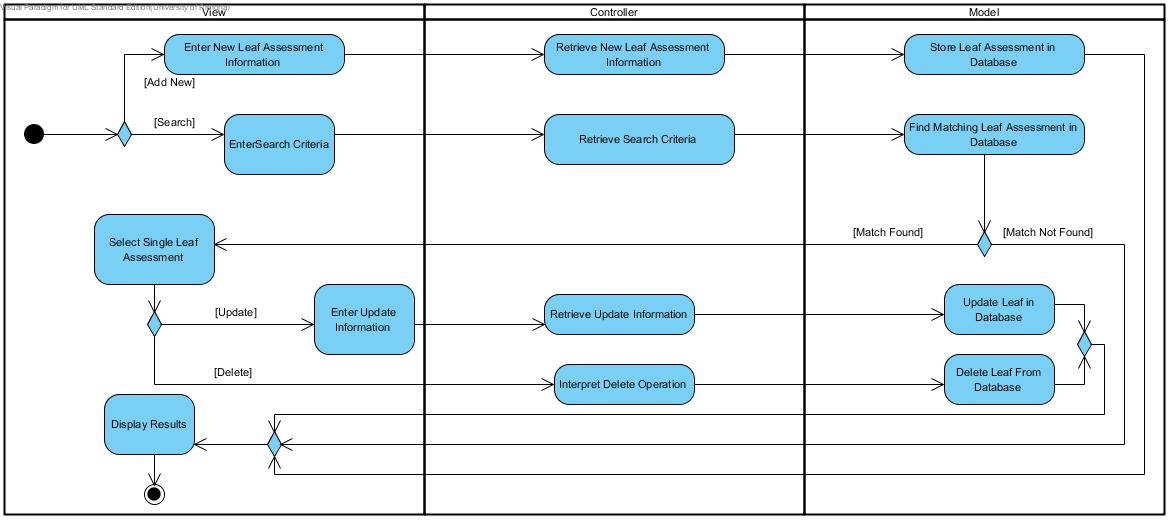
\includegraphics[width=2in, height=2in]{Pictures/LeafAssesmentActivityDiagram.jpg}
										\caption{Leaf Assessment Activity Diagram}
						\end{figure}
						\begin{figure}[h]
										\centering
										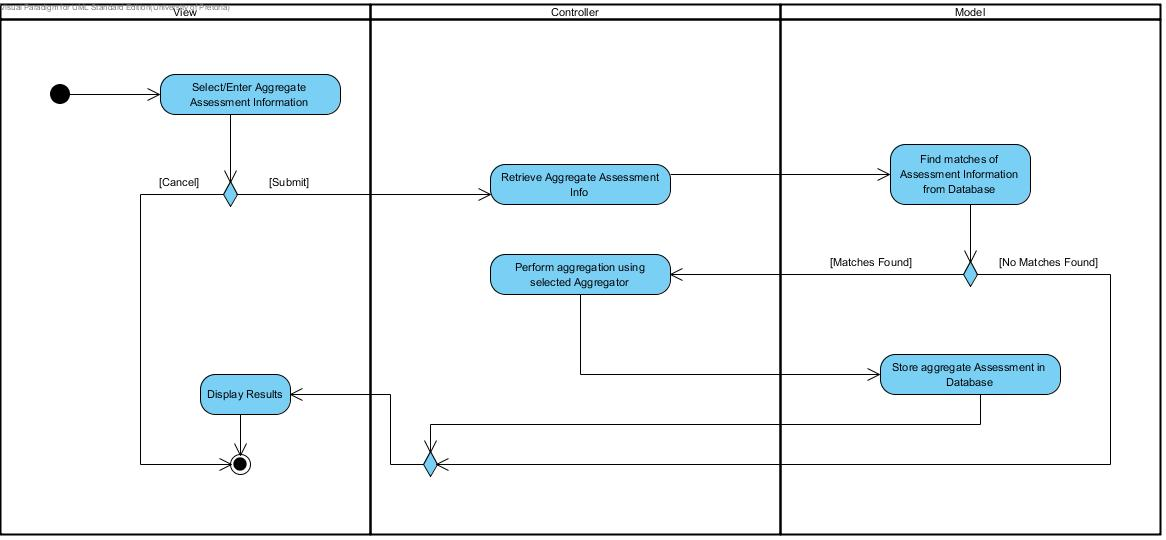
\includegraphics[width=2in, height=2in]{Pictures/AggregateAssesmentActivityDiagram.jpg}
										\caption{Aggregate Assessment Activity Diagram}
						\end{figure}
						\begin{figure}[h]
										\centering
										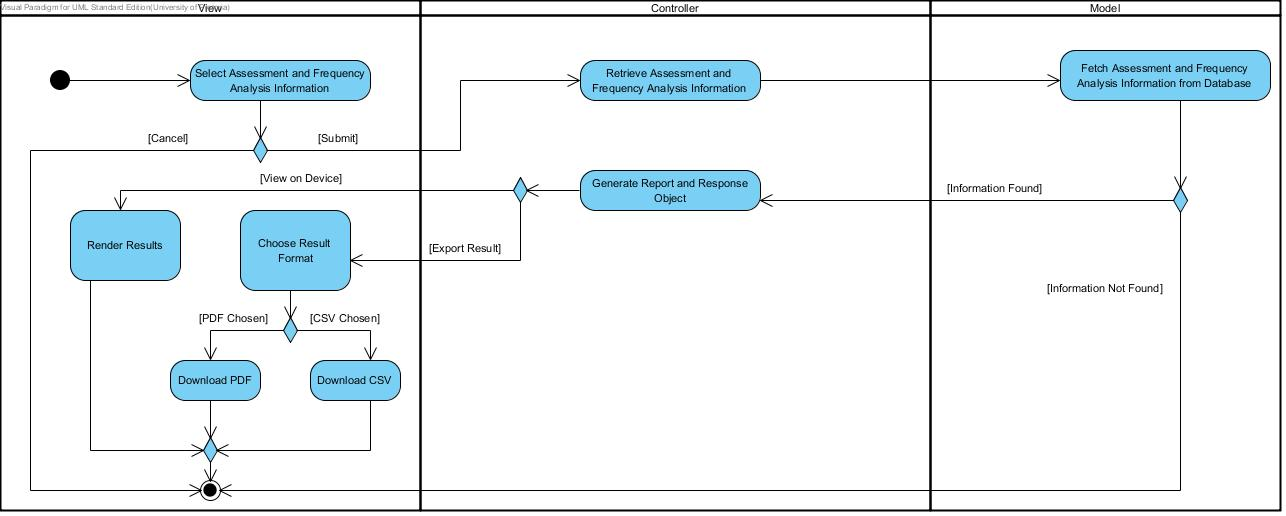
\includegraphics[width=2in, height=2in]{Pictures/AssessmentReportActivityDiagram.jpg}
										\caption{Assessment Report Activity Diagram}
						\end{figure}
						\begin{figure}[h]
										\centering
										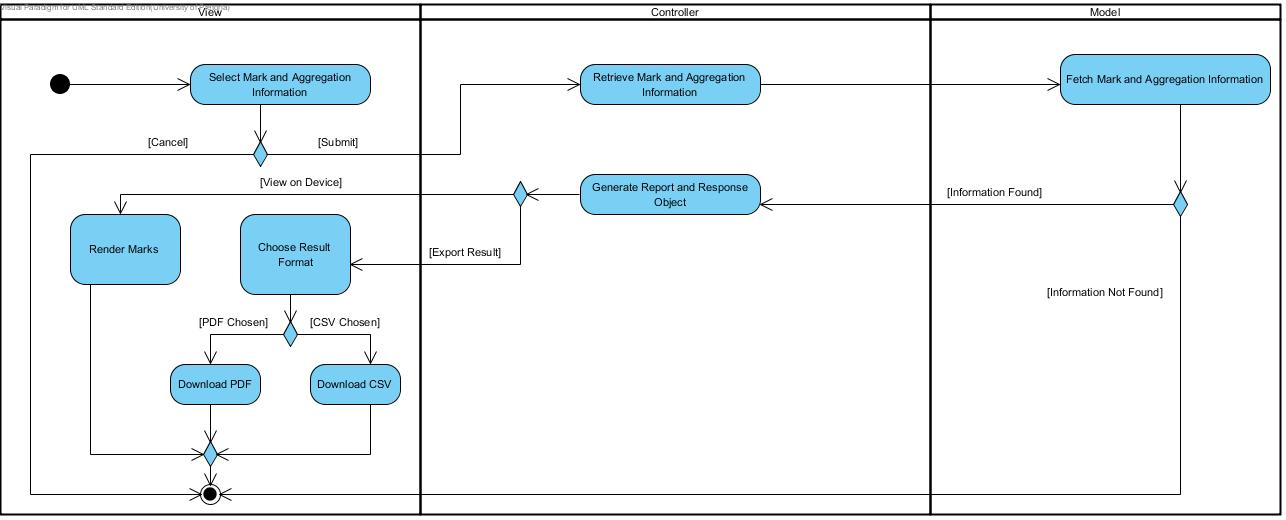
\includegraphics[width=2in, height=2in]{Pictures/StudentMarksReport.jpg}
										\caption{Student Marks Report Activity Diagram}
						\end{figure}
						\begin{figure}[h]
										\centering
										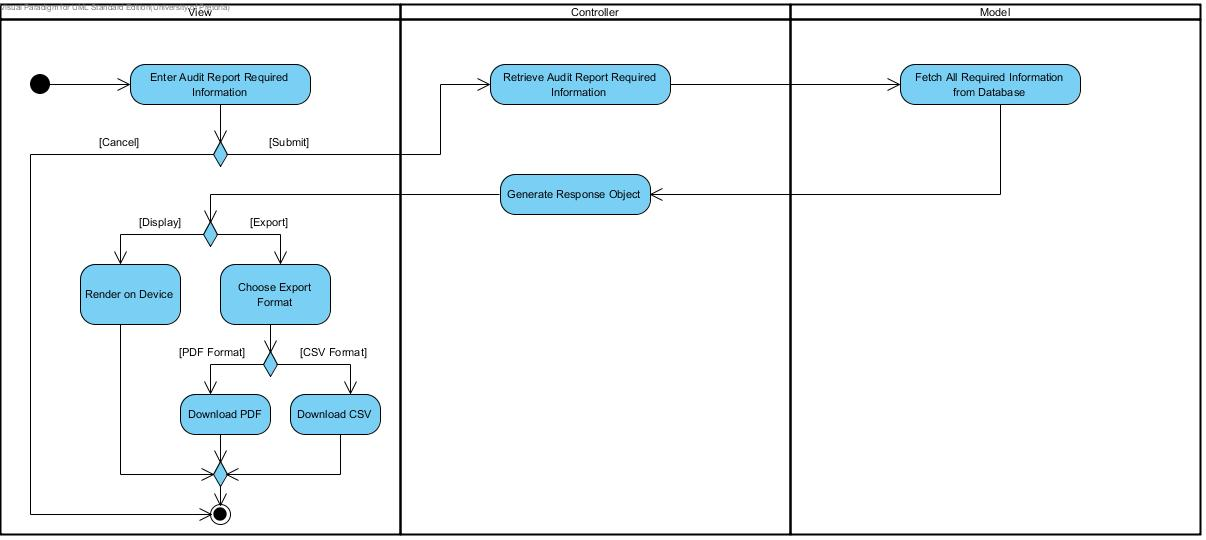
\includegraphics[width=2in, height=2in]{Pictures/AuditReportActivityDiagram.jpg}
										\caption{Audit Report Activity Diagram}
						\end{figure}
				\vspace{0.2in}
		
		\subsection{User Interface Designs} %MatthewHughes and Ndivhuwo Nthambeleni
						%This includes work-flow specifications
				\vspace{0.2in}
		
		\subsection{Database Desgin} %MatthewHughes and Mbulungo Musetsho
						%Database tables, etc
						
				\vspace{0.2in}
			
			
	
	\section{Open Issues}
	
		\vspace{0.2in}
		
		
	\newpage
	\section{Glossary}
	
		\vspace{0.2in}
		
			
	
	
\end{document}
